\documentclass[12pt,a4paper]{article}

% Paquetes
\usepackage[utf8]{inputenc}
\usepackage[spanish]{babel}
\usepackage{geometry}
\geometry{margin=2.5cm}
\usepackage{graphicx}
\usepackage{booktabs}
\usepackage{amsmath}
\usepackage{hyperref}
\usepackage{float}
\usepackage{listings}
\usepackage{xcolor}
\usepackage{caption}
\usepackage{subcaption}
\usepackage{fancyhdr}
\usepackage{parskip}

% Configuración de listings para Python
\lstset{
    language=Python,
    basicstyle=\ttfamily\footnotesize,
    keywordstyle=\color{blue}\bfseries,
    stringstyle=\color{red},
    commentstyle=\color{gray}\itshape,
    numbers=left,
    numberstyle=\tiny\color{gray},
    numbersep=5pt,
    frame=single,
    breaklines=true,
    breakatwhitespace=true,
    tabsize=4,
    showstringspaces=false,
    captionpos=b
}

% Encabezado
\pagestyle{fancy}
\fancyhf{}
\fancyhead[L]{Machine Learning -- Clasificación Binaria}
\fancyhead[R]{Universidad Complutense de Madrid}
\fancyfoot[C]{\thepage}

\title{\textbf{Trabajo de Clasificación Binaria} \\ \large Módulo: Machine Learning \\ \large Máster NTIC}
\author{Hassan Khan Asghar}
\date{Abril 2026}

\begin{document}

\maketitle
\thispagestyle{empty}

\begin{abstract}
En este trabajo se aborda un problema de clasificación binaria: predecir si un vehículo de segunda mano debe pintarse de color blanco o negro, a partir de sus características técnicas y comerciales. Se aplican tres técnicas de aprendizaje supervisado --- Árboles de Decisión, Random Forest y XGBoost --- siguiendo la metodología de análisis, búsqueda paramétrica, validación cruzada y comparación de modelos presentada en el módulo. Se utiliza la base de datos \texttt{datos\_tarea25.xlsx}, derivada del dataset \emph{Car Price Prediction Challenge} de Kaggle.
\end{abstract}

\tableofcontents
\newpage

% =====================================================================
\section{Análisis y depuración de la base de datos}
% =====================================================================

\subsection{Descripción del dataset}

La base de datos contiene 4340 observaciones y 15 variables relativas a vehículos de segunda mano. La variable dependiente es \texttt{Color} (White/Black), que se transforma en una variable binaria \texttt{target}: 1 si el coche es blanco, 0 si es negro.

Las variables independientes son: \textit{Price} (precio de venta), \textit{Levy} (impuestos), \textit{Manufacturer} (fabricante), \textit{Prod.\ year} (año de fabricación), \textit{Category} (categoría del vehículo), \textit{Leather interior} (interior de cuero), \textit{Fuel type} (tipo de combustible), \textit{Engine volume} (volumen del motor), \textit{Mileage} (kilometraje), \textit{Cylinders} (cilindros), \textit{Gear box type} (tipo de caja de cambios), \textit{Drive wheels} (ruedas motrices), \textit{Wheel} (posición del volante) y \textit{Airbags} (número de airbags).

\subsection{Proceso de depuración}

\subsubsection{Eliminación de duplicados}

Se detectaron \textbf{1534 filas duplicadas} (35.3\% del total), que fueron eliminadas. Tras la limpieza, el dataset queda con 2806 observaciones. La distribución de la variable objetivo es razonablemente equilibrada: 51.2\% Black y 48.8\% White.

\subsubsection{Variable \texttt{Levy}}

Esta variable contiene valores numéricos almacenados como texto, con 634 observaciones que presentan el carácter ``-'' como valor faltante. Se convirtió a numérico y se imputaron los valores faltantes con la \textbf{mediana} (781.0), al ser una medida robusta frente a valores extremos.

\begin{lstlisting}[caption={Tratamiento de Levy}]
df['Levy'] = df['Levy'].replace('-', np.nan)
df['Levy'] = pd.to_numeric(df['Levy'])
df['Levy'] = df['Levy'].fillna(df['Levy'].median())
\end{lstlisting}

\subsubsection{Variable \texttt{Engine volume}}

Contiene valores como ``2.0 Turbo'' que combinan información numérica (volumen) y categórica (turbo). Se separaron en dos variables: el volumen numérico y una variable binaria \texttt{Turbo} (1 si el motor es turbo, 0 en caso contrario). Solo 178 vehículos (6.3\%) disponen de motor turbo.

\begin{lstlisting}[caption={Separación de Engine volume y Turbo}]
df['Turbo'] = df['Engine volume'].str.contains('Turbo').astype(int)
df['Engine volume'] = df['Engine volume'].str.replace(' Turbo', '')
df['Engine volume'] = pd.to_numeric(df['Engine volume'])
\end{lstlisting}

\subsubsection{Variable \texttt{Mileage}}

Almacenada como texto con el sufijo `` km''. Se eliminó el sufijo y se convirtió a numérico.

\subsubsection{Variables binarias}

\texttt{Leather interior} (Yes/No) y \texttt{Wheel} (Left wheel/Right-hand drive) se convirtieron en variables binarias (0/1) directamente, al tener solo dos categorías.

\subsubsection{Variables categóricas multi-nivel}

Las variables \texttt{Manufacturer} (4 categorías), \texttt{Category} (3), \texttt{Fuel type} (3), \texttt{Gear box type} (2) y \texttt{Drive wheels} (3) se codificaron mediante \textit{one-hot encoding} con \texttt{pd.get\_dummies(drop\_first=True)} para evitar multicolinealidad (se elimina la primera categoría como referencia).

\begin{lstlisting}[caption={One-hot encoding de variables categóricas}]
cat_cols = ['Manufacturer', 'Category', 'Fuel type',
            'Gear box type', 'Drive wheels']
df = pd.get_dummies(df, columns=cat_cols, drop_first=True, dtype=int)
\end{lstlisting}

\subsection{Justificación del Feature Engineering para los modelos}

\textbf{Para árboles de decisión, Random Forest y XGBoost:}
\begin{itemize}
    \item \textbf{No se requiere escalado}: los modelos basados en árboles son invariantes a transformaciones monótonas de las variables, ya que trabajan con puntos de corte.
    \item \textbf{One-hot encoding es necesario}: aunque los árboles pueden manejar variables categóricas ordinales, la implementación de scikit-learn requiere variables numéricas. El \texttt{drop\_first=True} no es estrictamente necesario para árboles (no sufren multicolinealidad como los modelos lineales), pero es una buena práctica que reduce la dimensionalidad.
    \item \textbf{Imputación de Levy}: se opta por la mediana al ser robusta frente a los valores atípicos observados en la distribución de esta variable.
    \item \textbf{Separación de Turbo}: captura información cualitativa (tipo de motor) que de otro modo quedaría mezclada con la cuantitativa (volumen).
\end{itemize}

\subsection{Análisis exploratorio}

\begin{figure}[H]
    \centering
    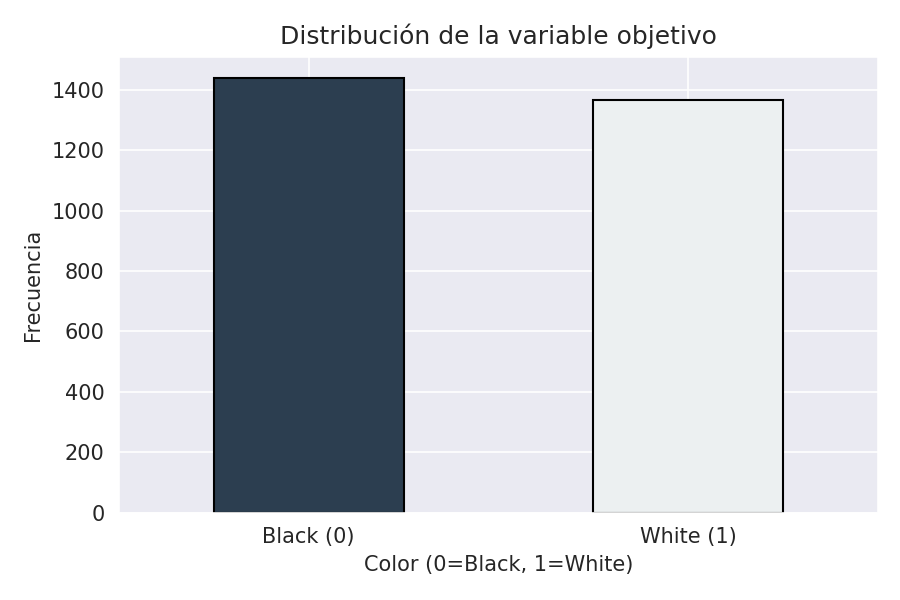
\includegraphics[width=0.55\textwidth]{figuras/fig01_distribucion_target.png}
    \caption{Distribución de la variable objetivo. Las clases están razonablemente equilibradas.}
    \label{fig:dist_target}
\end{figure}

\begin{figure}[H]
    \centering
    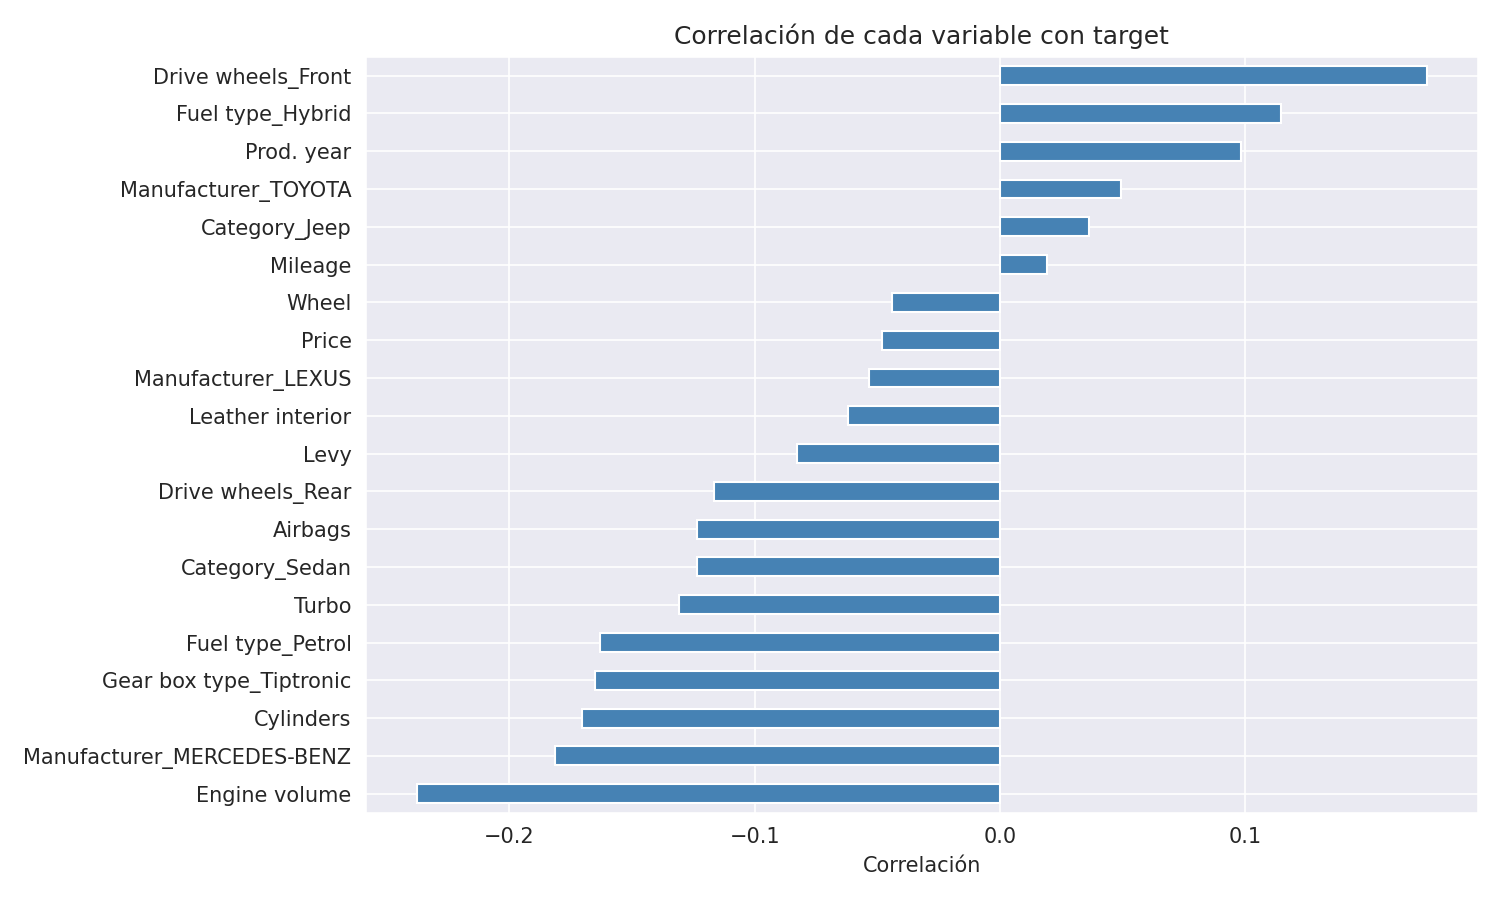
\includegraphics[width=0.7\textwidth]{figuras/fig03_correlacion_target.png}
    \caption{Correlación de cada variable con la variable objetivo.}
    \label{fig:corr_target}
\end{figure}

El dataset final cuenta con \textbf{20 variables predictoras} y 2806 observaciones. Se realizó una partición \textbf{80/20} estratificada (train: 2244, test: 562), verificando que la distribución de la variable objetivo se mantenga similar en ambos conjuntos (51.2\%/48.8\% en ambos).

\begin{lstlisting}[caption={División train/test estratificada}]
X_train, X_test, y_train, y_test = train_test_split(
    X, y, test_size=0.2, random_state=123, stratify=y)
\end{lstlisting}

\newpage
% =====================================================================
\section{Búsqueda paramétrica del mejor Árbol de Decisión}
% =====================================================================

\subsection{Configuración de la búsqueda}

Se realizó una búsqueda exhaustiva (\texttt{GridSearchCV}) sobre el espacio de hiperparámetros del \texttt{DecisionTreeClassifier}, evaluando simultáneamente \textbf{cuatro métricas de validación} de la bondad de la clasificación:

\begin{enumerate}
    \item \textbf{Accuracy}: proporción de predicciones correctas.
    \item \textbf{Precision (macro)}: media de la precisión por clase, sin ponderar por tamaño.
    \item \textbf{Recall (macro)}: media de la sensibilidad por clase.
    \item \textbf{F1-Score (macro)}: media armónica de precision y recall por clase.
\end{enumerate}

El espacio de hiperparámetros explorado fue:

\begin{table}[H]
\centering
\caption{Grid de hiperparámetros para el Árbol de Decisión}
\begin{tabular}{ll}
\toprule
\textbf{Hiperparámetro} & \textbf{Valores} \\
\midrule
\texttt{max\_depth} & 2, 3, 5, 10, 15, 20 \\
\texttt{min\_samples\_split} & 5, 10, 20, 50, 100 \\
\texttt{min\_samples\_leaf} & 3, 10, 30, 50 \\
\texttt{criterion} & gini, entropy \\
\bottomrule
\end{tabular}
\end{table}

Esto genera un total de $6 \times 5 \times 4 \times 2 = 240$ combinaciones, evaluadas con validación cruzada estratificada de 4 folds (\texttt{StratifiedKFold}).

\begin{lstlisting}[caption={GridSearchCV con 4 métricas de validación}]
scoring_metrics = ['accuracy', 'precision_macro', 'recall_macro', 'f1_macro']
cv = StratifiedKFold(n_splits=4, shuffle=True, random_state=123)
dt_grid = GridSearchCV(estimator=DecisionTreeClassifier(random_state=123),
                       param_grid=dt_param_grid, cv=cv,
                       scoring=scoring_metrics, refit='accuracy')
dt_grid.fit(X_train, y_train)
\end{lstlisting}

\subsection{Resultados}

El mejor árbol según las cuatro métricas de forma consistente es:
\begin{itemize}
    \item \texttt{criterion}: gini
    \item \texttt{max\_depth}: 3
    \item \texttt{min\_samples\_leaf}: 50
    \item Accuracy CV: \textbf{0.6373}, Precision macro: 0.6383, Recall macro: 0.6373, F1 macro: 0.6365
\end{itemize}

Es notable que el mismo modelo ocupa las primeras posiciones en las cuatro métricas, lo que indica que para este problema, las métricas están altamente correlacionadas dado el equilibrio de clases.

\subsubsection{Análisis de sobreajuste}

\begin{table}[H]
\centering
\caption{Accuracy en train vs.\ test para el mejor Árbol de Decisión}
\begin{tabular}{lcc}
\toprule
& \textbf{Train} & \textbf{Test} \\
\midrule
Accuracy & 0.6453 & 0.6299 \\
\bottomrule
\end{tabular}
\end{table}

La diferencia es mínima (1.5\%), lo que indica que el modelo \textbf{no presenta sobreajuste}. Esto es coherente con la profundidad limitada (\texttt{max\_depth=3}) y el tamaño mínimo de hoja elevado (\texttt{min\_samples\_leaf=50}).

\begin{figure}[H]
    \centering
    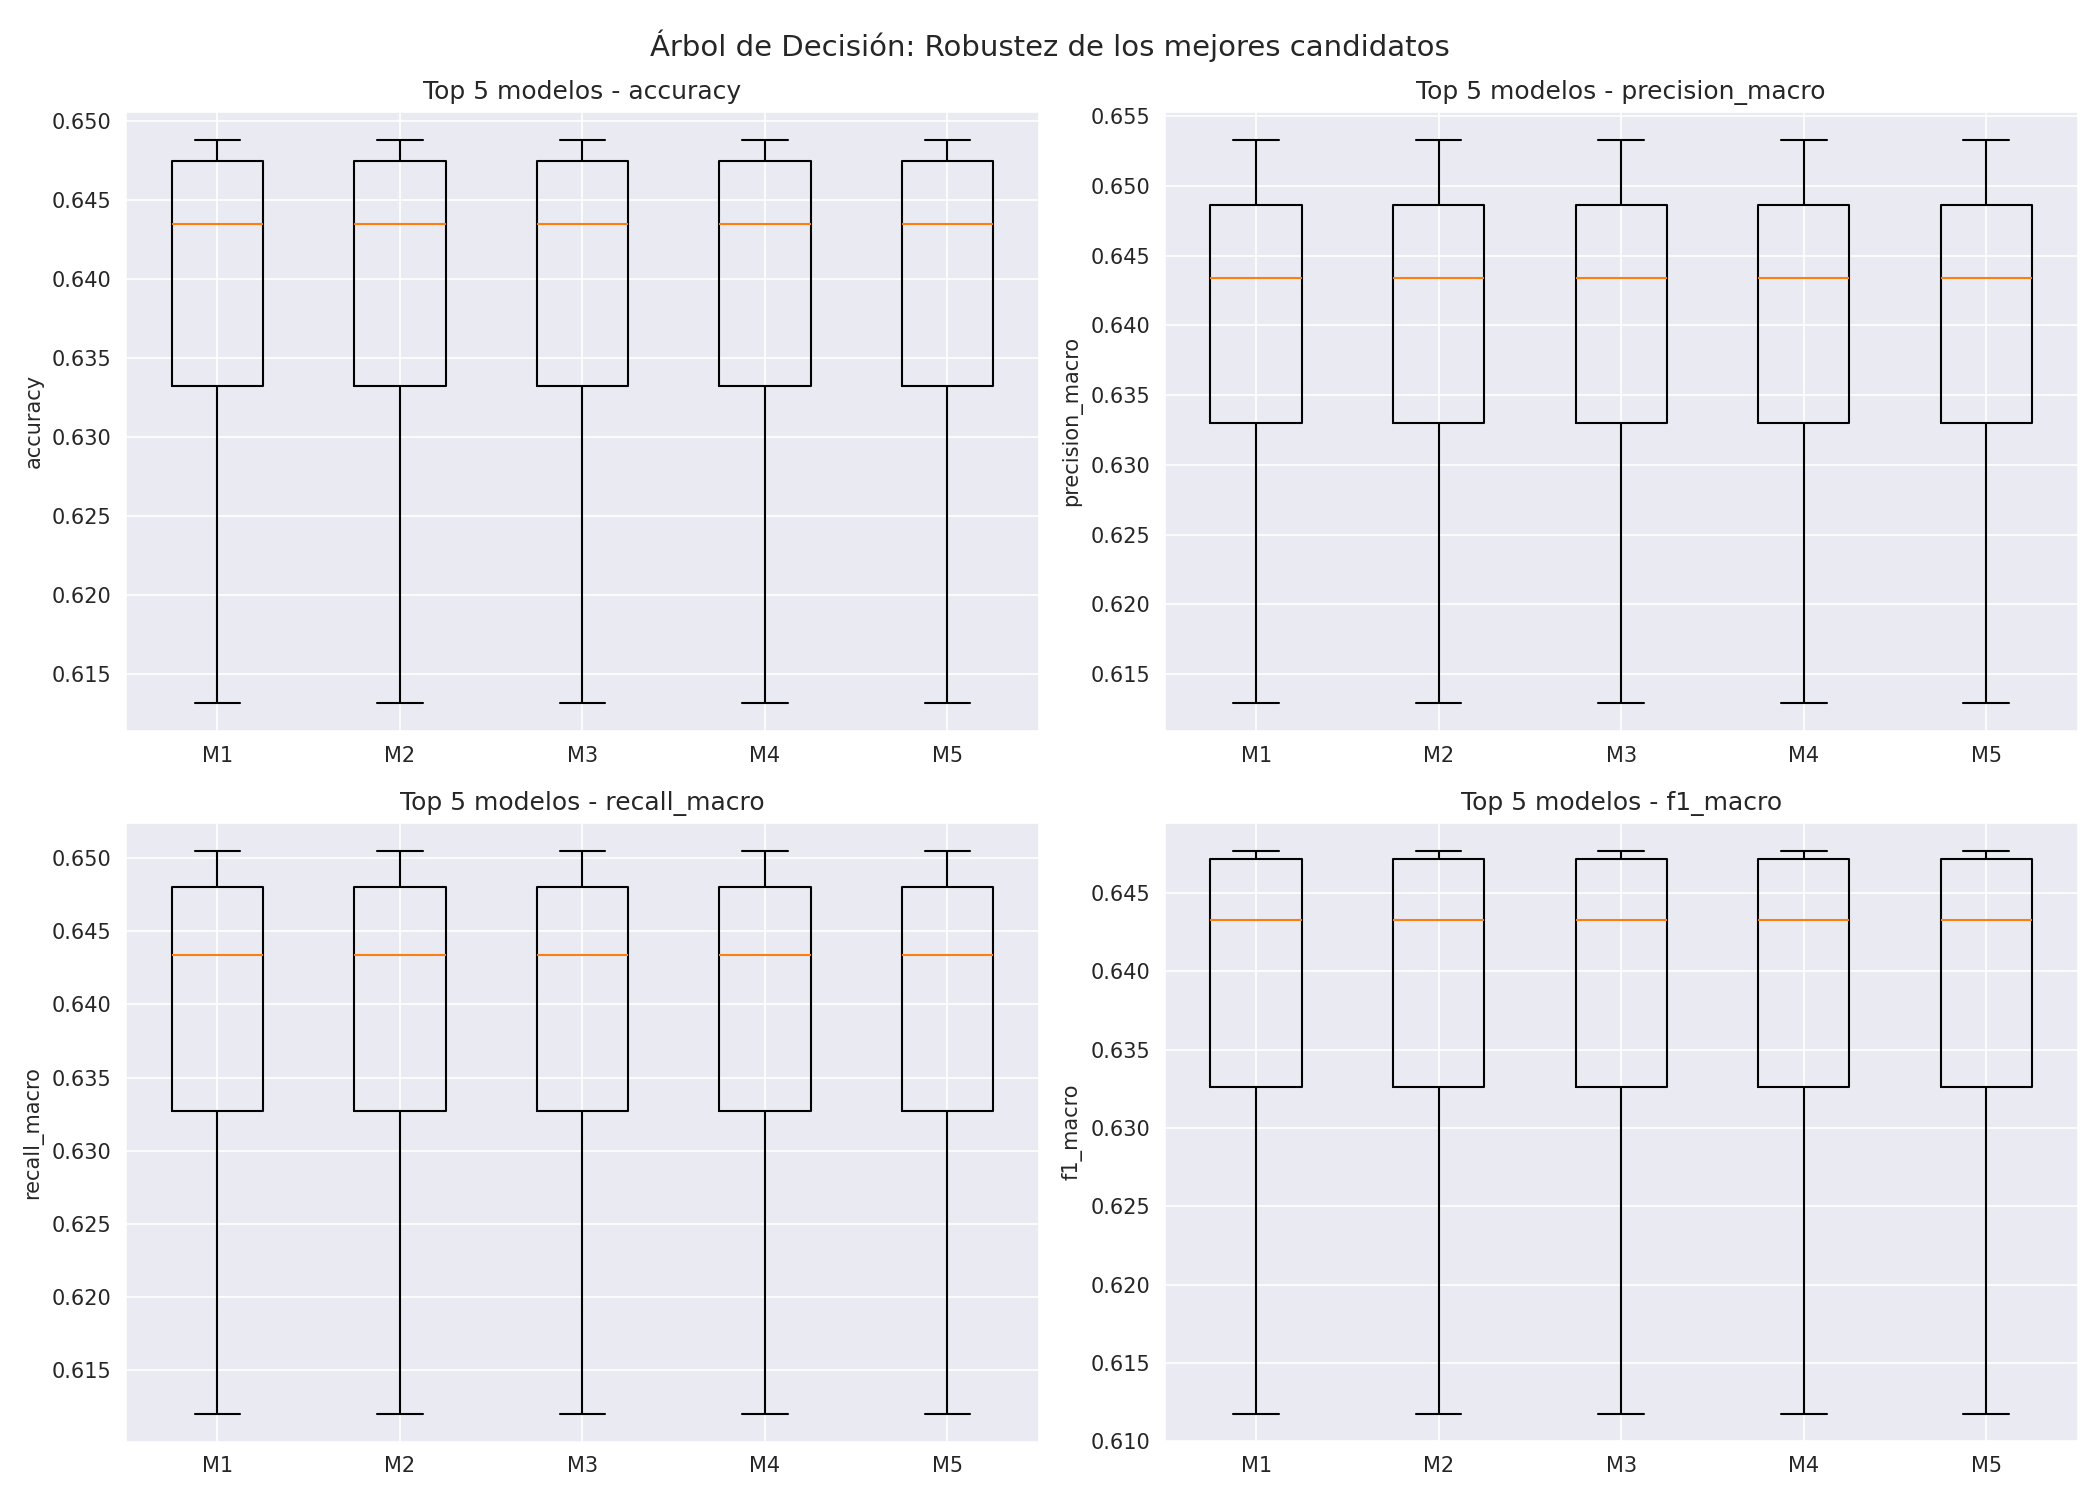
\includegraphics[width=0.85\textwidth]{figuras/fig04_dt_boxplots_robustez.png}
    \caption{Boxplots de robustez de los top 5 candidatos según cada métrica. Se observa poca variabilidad entre folds, indicando estabilidad del modelo.}
    \label{fig:dt_robustez}
\end{figure}

\subsection{Representación gráfica del árbol ganador}

\begin{figure}[H]
    \centering
    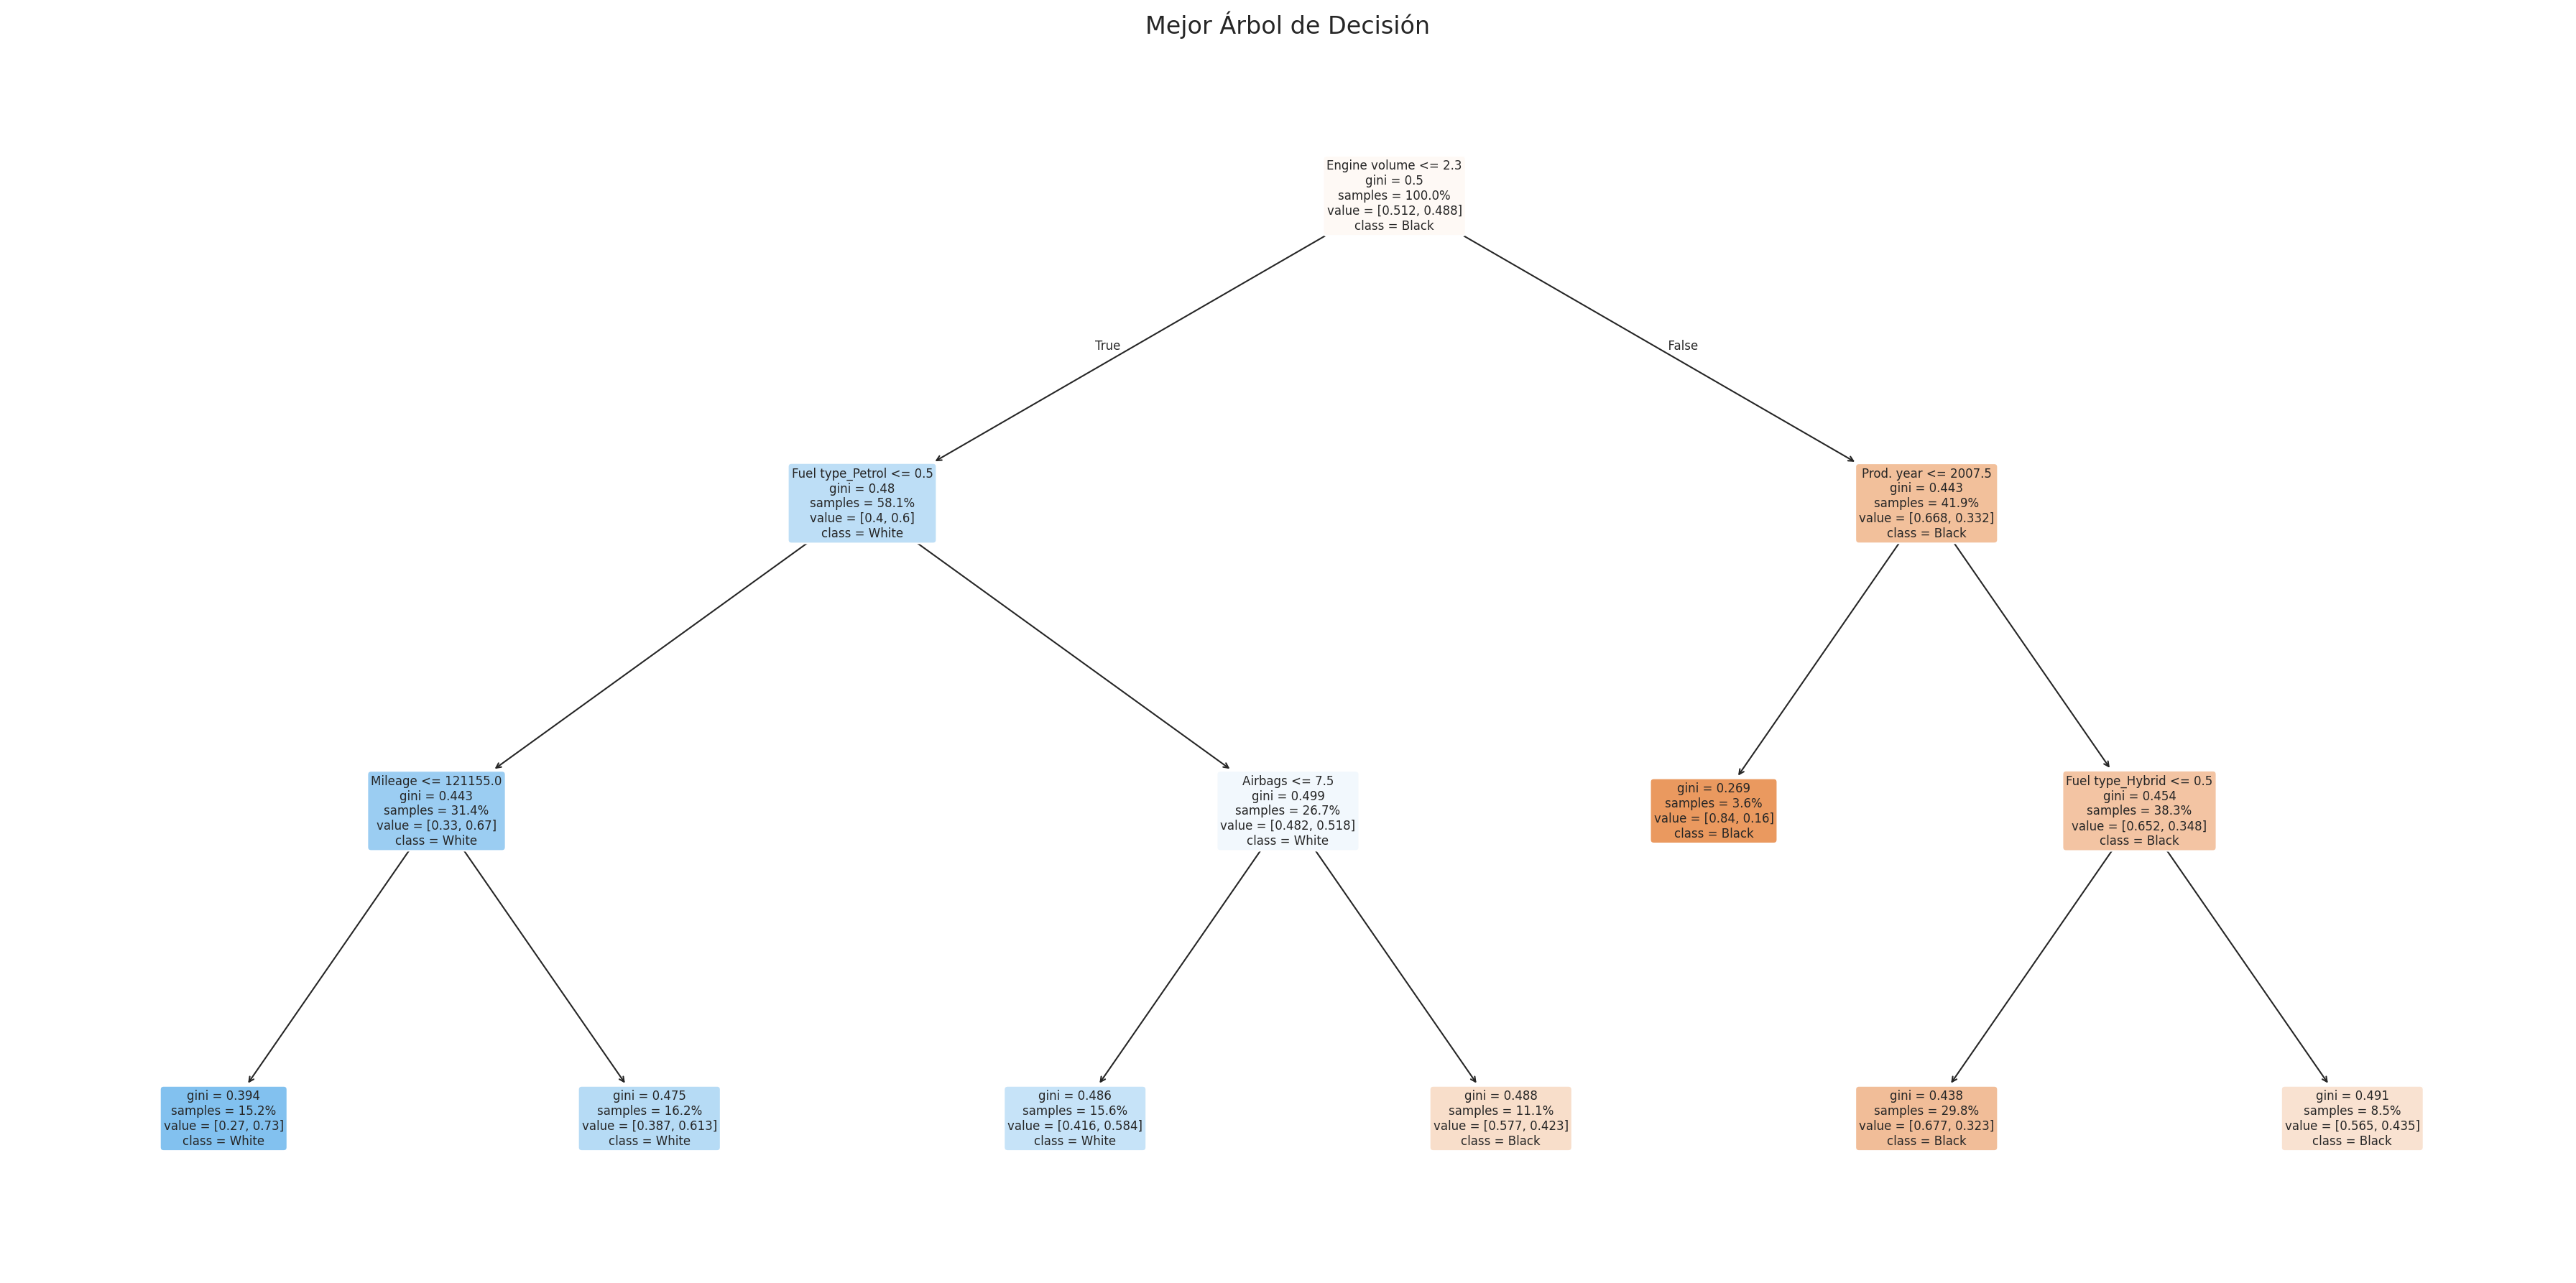
\includegraphics[width=\textwidth]{figuras/fig07_dt_tree_plot.png}
    \caption{Representación gráfica del mejor Árbol de Decisión.}
    \label{fig:dt_tree}
\end{figure}

\subsection{Reglas del árbol en formato texto}

\begin{verbatim}
|--- Engine volume <= 2.30
|   |--- Fuel type_Petrol <= 0.50
|   |   |--- class: White
|   |--- Fuel type_Petrol > 0.50
|   |   |--- Airbags <= 7.50
|   |   |   |--- class: White
|   |   |--- Airbags > 7.50
|   |   |   |--- class: Black
|--- Engine volume > 2.30
|   |--- Prod. year <= 2007.50
|   |   |--- class: Black
|   |--- Prod. year > 2007.50
|   |   |--- class: Black
\end{verbatim}

\textbf{Interpretación:} El árbol revela que el \textbf{volumen del motor} es la variable más discriminante. Los vehículos con motor $\leq 2.3$L tienden a ser blancos (salvo los de gasolina con muchos airbags), mientras que los de motor $> 2.3$L tienden a ser negros.

\subsection{Importancia de variables}

\begin{figure}[H]
    \centering
    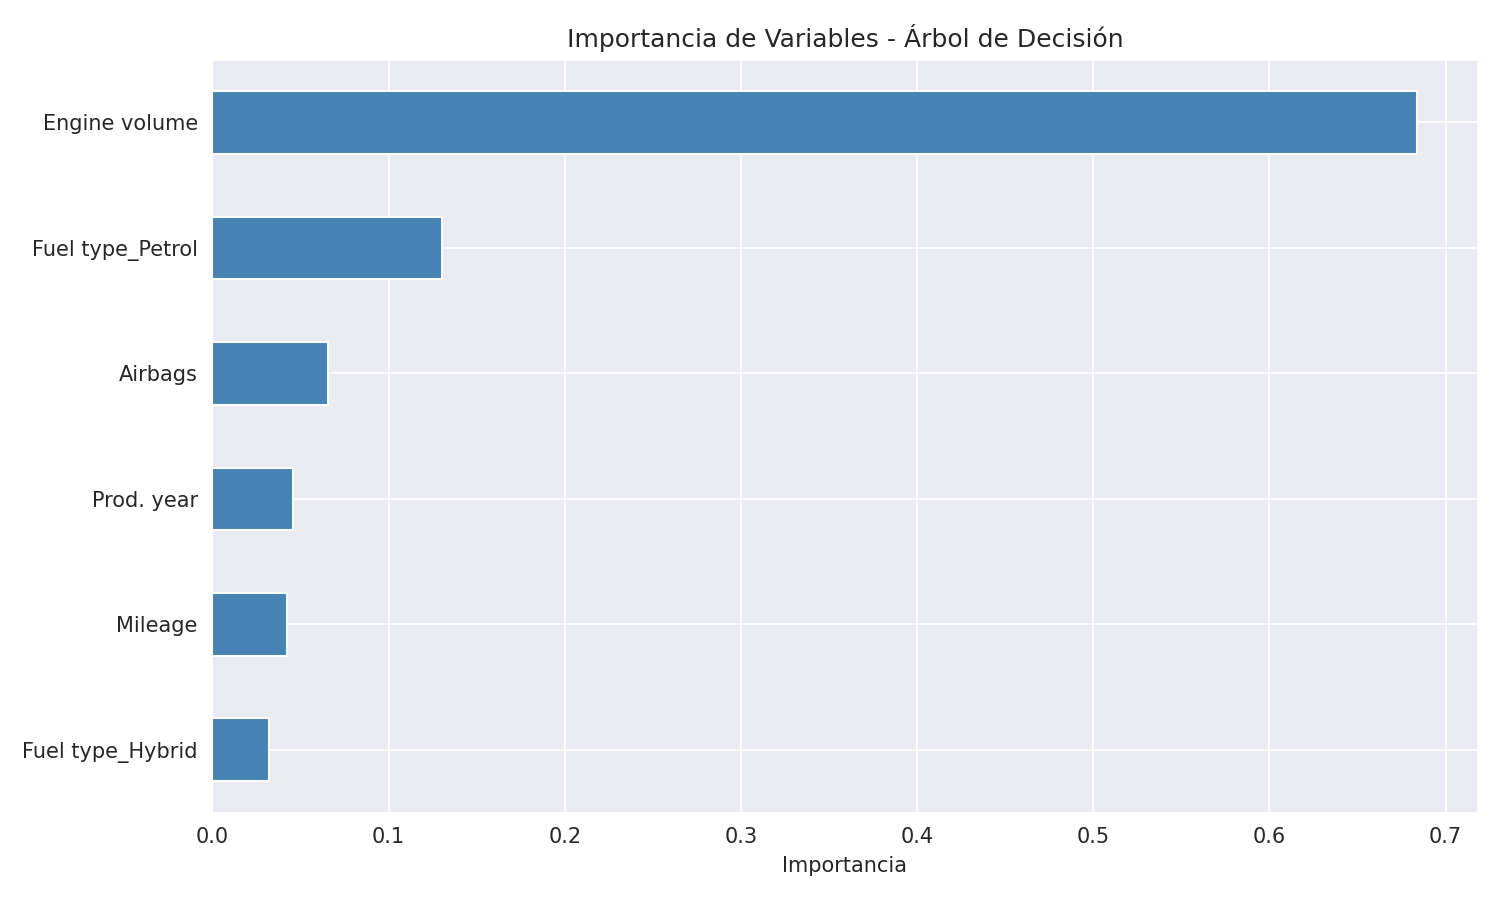
\includegraphics[width=0.7\textwidth]{figuras/fig08_dt_feature_importance.png}
    \caption{Importancia de variables en el Árbol de Decisión. \texttt{Engine volume} domina con un 68.4\% de importancia.}
    \label{fig:dt_importance}
\end{figure}

\newpage
% =====================================================================
\section{Búsqueda paramétrica de Random Forest y XGBoost}
% =====================================================================

\subsection{Random Forest}

\subsubsection{Configuración}

\begin{table}[H]
\centering
\caption{Grid de hiperparámetros para Random Forest}
\begin{tabular}{ll}
\toprule
\textbf{Hiperparámetro} & \textbf{Valores} \\
\midrule
\texttt{n\_estimators} & 50, 100, 200, 300 \\
\texttt{max\_depth} & 3, 5, 10, 15, 20 \\
\texttt{min\_samples\_split} & 5, 10, 20, 50 \\
\texttt{min\_samples\_leaf} & 3, 10, 30 \\
\texttt{criterion} & gini, entropy \\
\bottomrule
\end{tabular}
\end{table}

Total: 480 combinaciones evaluadas con \texttt{StratifiedKFold(4)}, optimizando según \textbf{Accuracy}.

\subsubsection{Resultados}

\begin{itemize}
    \item \textbf{Mejores parámetros}: \texttt{criterion}=entropy, \texttt{max\_depth}=20, \texttt{min\_samples\_leaf}=3, \texttt{min\_samples\_split}=10, \texttt{n\_estimators}=300
    \item \textbf{Accuracy CV}: 0.6662
    \item \textbf{Accuracy Test}: 0.6584
    \item \textbf{Accuracy Train}: 0.8373
\end{itemize}

Se observa una diferencia notable entre train (83.7\%) y test (65.8\%), lo que indica \textbf{sobreajuste}. El modelo es más complejo que el árbol individual (profundidad 20, hojas mínimas de 3), lo cual le permite memorizar patrones del entrenamiento. No obstante, la accuracy en test sigue siendo la más alta de los tres modelos.

\begin{figure}[H]
    \centering
    \begin{subfigure}[b]{0.48\textwidth}
        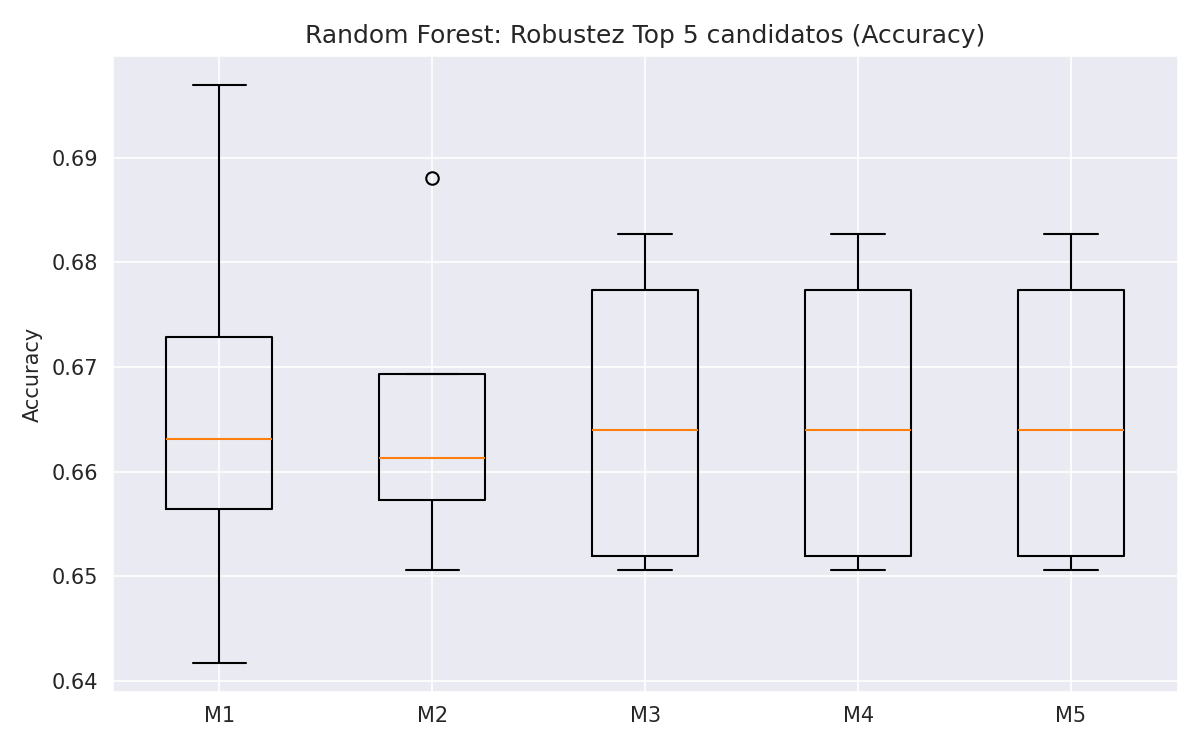
\includegraphics[width=\textwidth]{figuras/fig09_rf_boxplots_robustez.png}
        \caption{Robustez de los top 5 candidatos}
    \end{subfigure}
    \hfill
    \begin{subfigure}[b]{0.48\textwidth}
        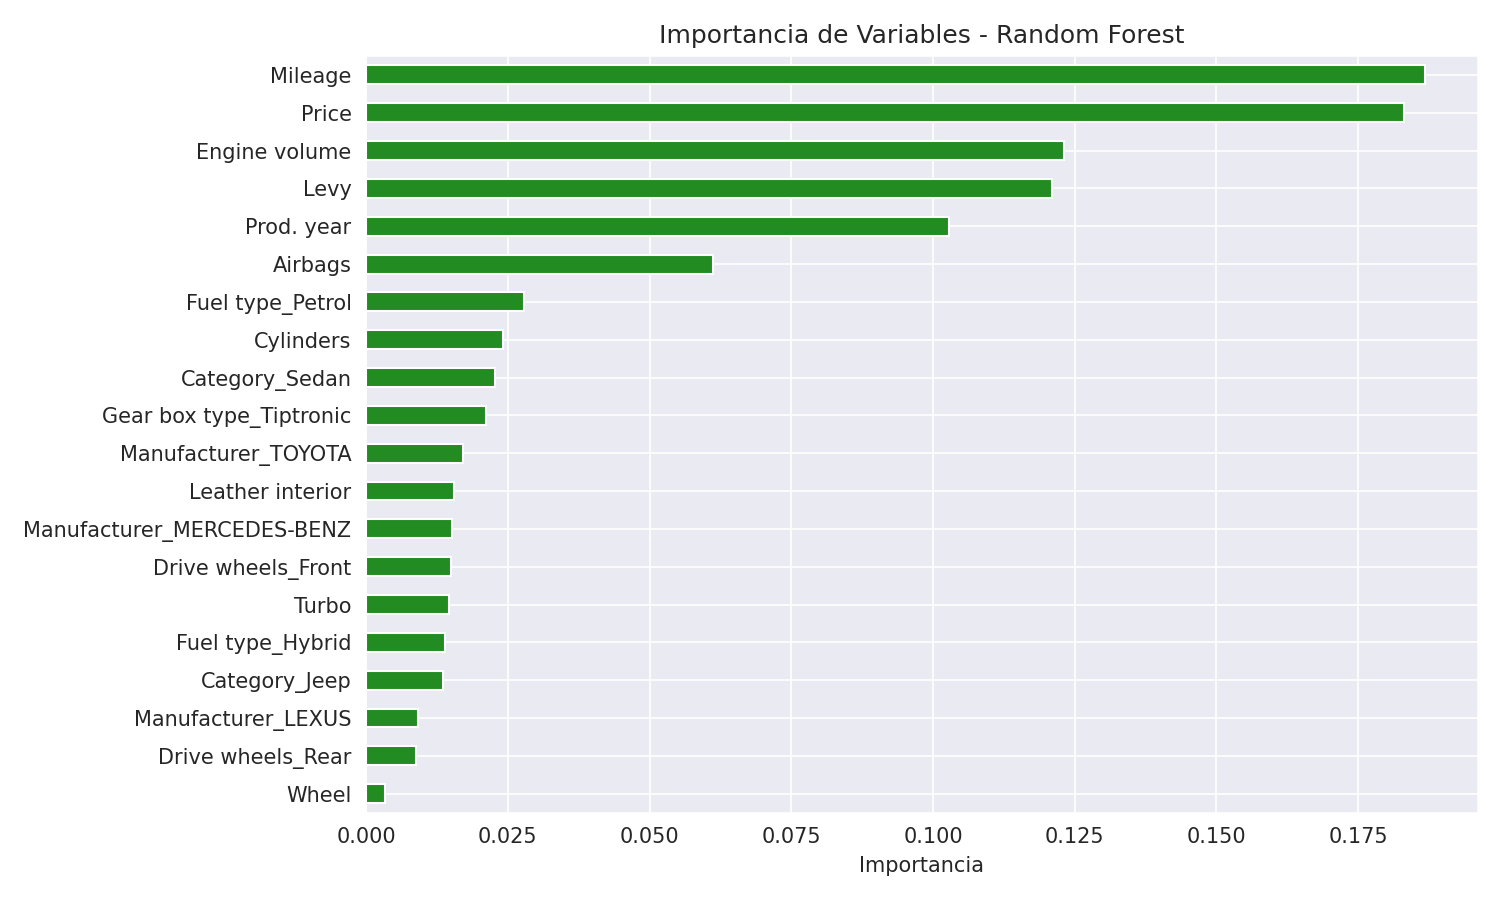
\includegraphics[width=\textwidth]{figuras/fig10_rf_feature_importance.png}
        \caption{Importancia de variables}
    \end{subfigure}
    \caption{Random Forest: análisis de robustez e importancia de variables.}
    \label{fig:rf_analysis}
\end{figure}

\subsection{XGBoost}

\subsubsection{Configuración}

\begin{table}[H]
\centering
\caption{Grid de hiperparámetros para XGBoost}
\begin{tabular}{ll}
\toprule
\textbf{Hiperparámetro} & \textbf{Valores} \\
\midrule
\texttt{n\_estimators} & 100, 200, 300 \\
\texttt{max\_depth} & 3, 5, 10 \\
\texttt{learning\_rate} ($\eta$) & 0.01, 0.1, 0.3 \\
\texttt{gamma} ($\gamma$) & 0, 0.1, 0.5 \\
\texttt{min\_child\_weight} & 1, 5, 10 \\
\texttt{subsample} & 0.8, 1.0 \\
\bottomrule
\end{tabular}
\end{table}

Total: 486 combinaciones. XGBoost utiliza \texttt{booster='gbtree'} y \texttt{tree\_method='hist'}.

\subsubsection{Resultados}

\begin{itemize}
    \item \textbf{Mejores parámetros}: $\gamma=0.5$, $\eta=0.1$, \texttt{max\_depth}=5, \texttt{min\_child\_weight}=1, \texttt{n\_estimators}=100, \texttt{subsample}=1.0
    \item \textbf{Accuracy CV}: 0.6596
    \item \textbf{Accuracy Test}: 0.6388
    \item \textbf{Accuracy Train}: 0.7923
\end{itemize}

XGBoost presenta menor sobreajuste que Random Forest (diferencia train-test de 15.3\% vs.\ 17.9\%), lo cual se atribuye a la regularización mediante $\gamma=0.5$.

\begin{figure}[H]
    \centering
    \begin{subfigure}[b]{0.48\textwidth}
        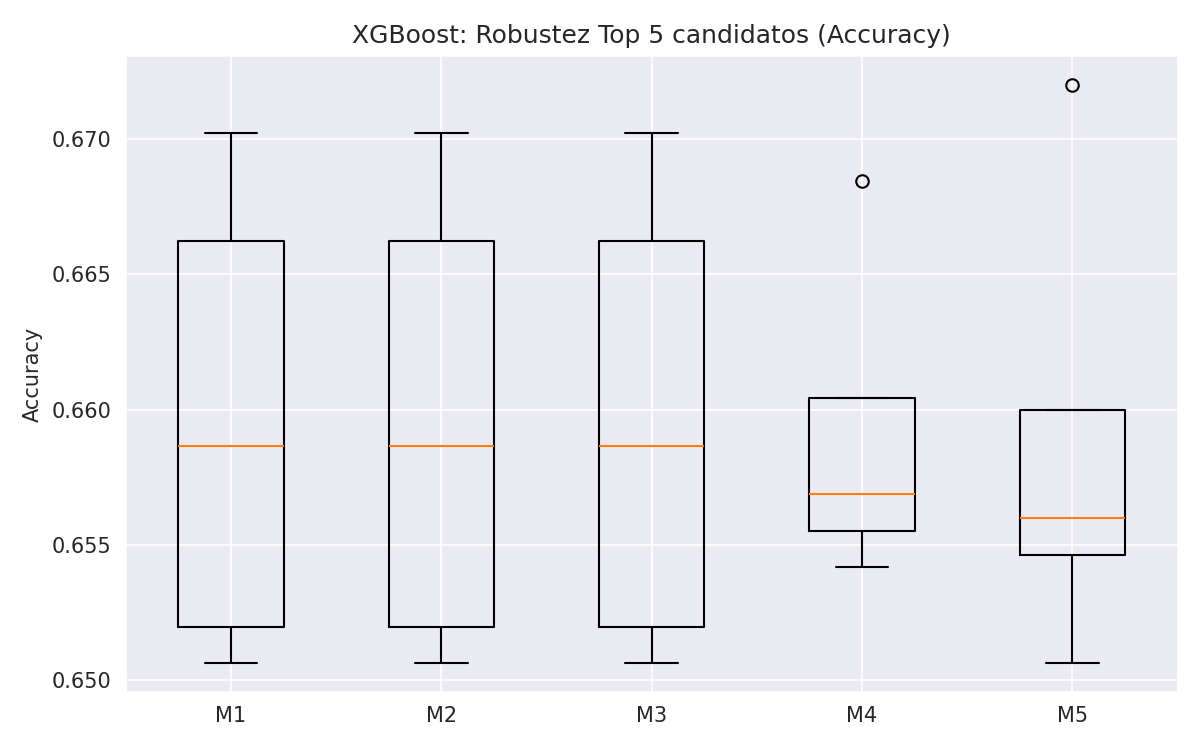
\includegraphics[width=\textwidth]{figuras/fig11_xgb_boxplots_robustez.png}
        \caption{Robustez de los top 5 candidatos}
    \end{subfigure}
    \hfill
    \begin{subfigure}[b]{0.48\textwidth}
        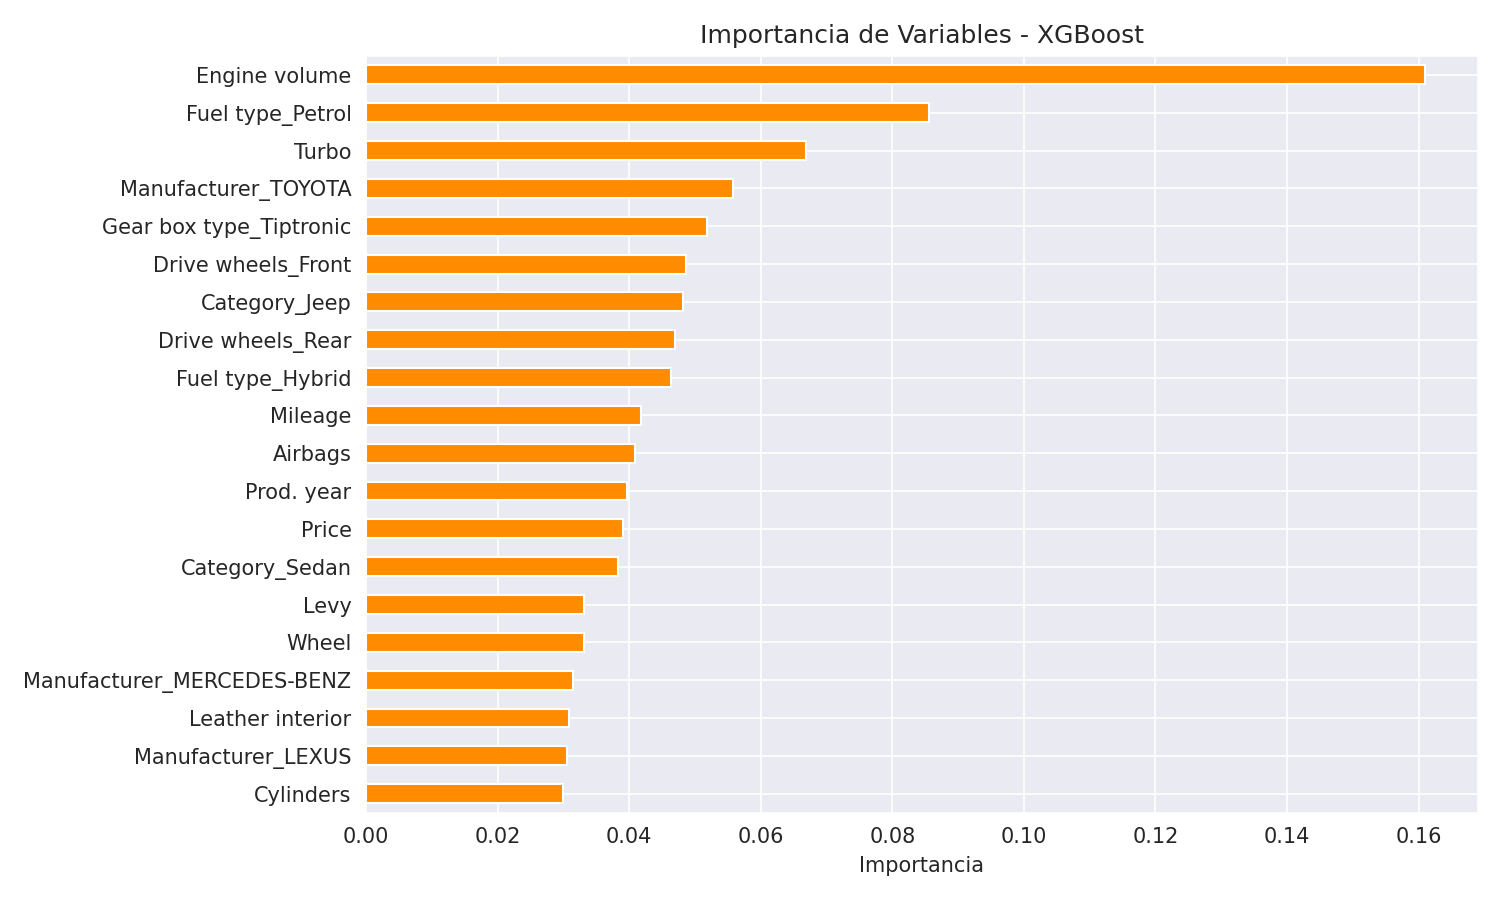
\includegraphics[width=\textwidth]{figuras/fig12_xgb_feature_importance.png}
        \caption{Importancia de variables}
    \end{subfigure}
    \caption{XGBoost: análisis de robustez e importancia de variables.}
    \label{fig:xgb_analysis}
\end{figure}

\newpage
% =====================================================================
\section{Comparación completa de modelos}
% =====================================================================

\subsection{Resumen de métricas en test}

\begin{table}[H]
\centering
\caption{Métricas de clasificación en el conjunto de test}
\begin{tabular}{lccccc}
\toprule
\textbf{Modelo} & \textbf{Accuracy} & \textbf{Precision} & \textbf{Recall} & \textbf{F1-Score} & \textbf{AUC} \\
\midrule
Árbol de Decisión & 0.6299 & 0.6260 & 0.5985 & 0.6119 & 0.6676 \\
Random Forest & \textbf{0.6584} & \textbf{0.6589} & \textbf{0.6204} & \textbf{0.6391} & \textbf{0.7165} \\
XGBoost & 0.6388 & 0.6403 & 0.5912 & 0.6148 & 0.7092 \\
\bottomrule
\end{tabular}
\end{table}

\textbf{Random Forest} obtiene los mejores resultados en todas las métricas en test.

\subsection{Análisis de sobreajuste}

\begin{table}[H]
\centering
\caption{Comparación train vs.\ test y análisis de sobreajuste}
\begin{tabular}{lcccc}
\toprule
\textbf{Modelo} & \textbf{Acc Train} & \textbf{Acc Test} & \textbf{Diferencia} & \textbf{Acc CV (media)} \\
\midrule
Árbol de Decisión & 0.6453 & 0.6299 & 0.0154 & 0.6373 \\
Random Forest & 0.8373 & 0.6584 & 0.1790 & 0.6662 \\
XGBoost & 0.7923 & 0.6388 & 0.1535 & 0.6596 \\
\bottomrule
\end{tabular}
\end{table}

El Árbol de Decisión es el modelo más estable (menor diferencia train-test), pero con menor capacidad predictiva. Random Forest y XGBoost presentan sobreajuste significativo, aunque su rendimiento generalizado sigue siendo superior.

\subsection{Validación cruzada repetida}

Para una evaluación más robusta, se realizó una validación cruzada repetida (\texttt{RepeatedStratifiedKFold}, 5 folds $\times$ 10 repeticiones = 50 evaluaciones):

\begin{table}[H]
\centering
\caption{Accuracy con validación cruzada repetida (5-fold $\times$ 10)}
\begin{tabular}{lcc}
\toprule
\textbf{Modelo} & \textbf{Media} & \textbf{Desv.\ Estándar} \\
\midrule
Árbol de Decisión & 0.6298 & $\pm$0.0208 \\
Random Forest & \textbf{0.6454} & $\pm$0.0184 \\
XGBoost & 0.6385 & $\pm$0.0232 \\
\bottomrule
\end{tabular}
\end{table}

\begin{figure}[H]
    \centering
    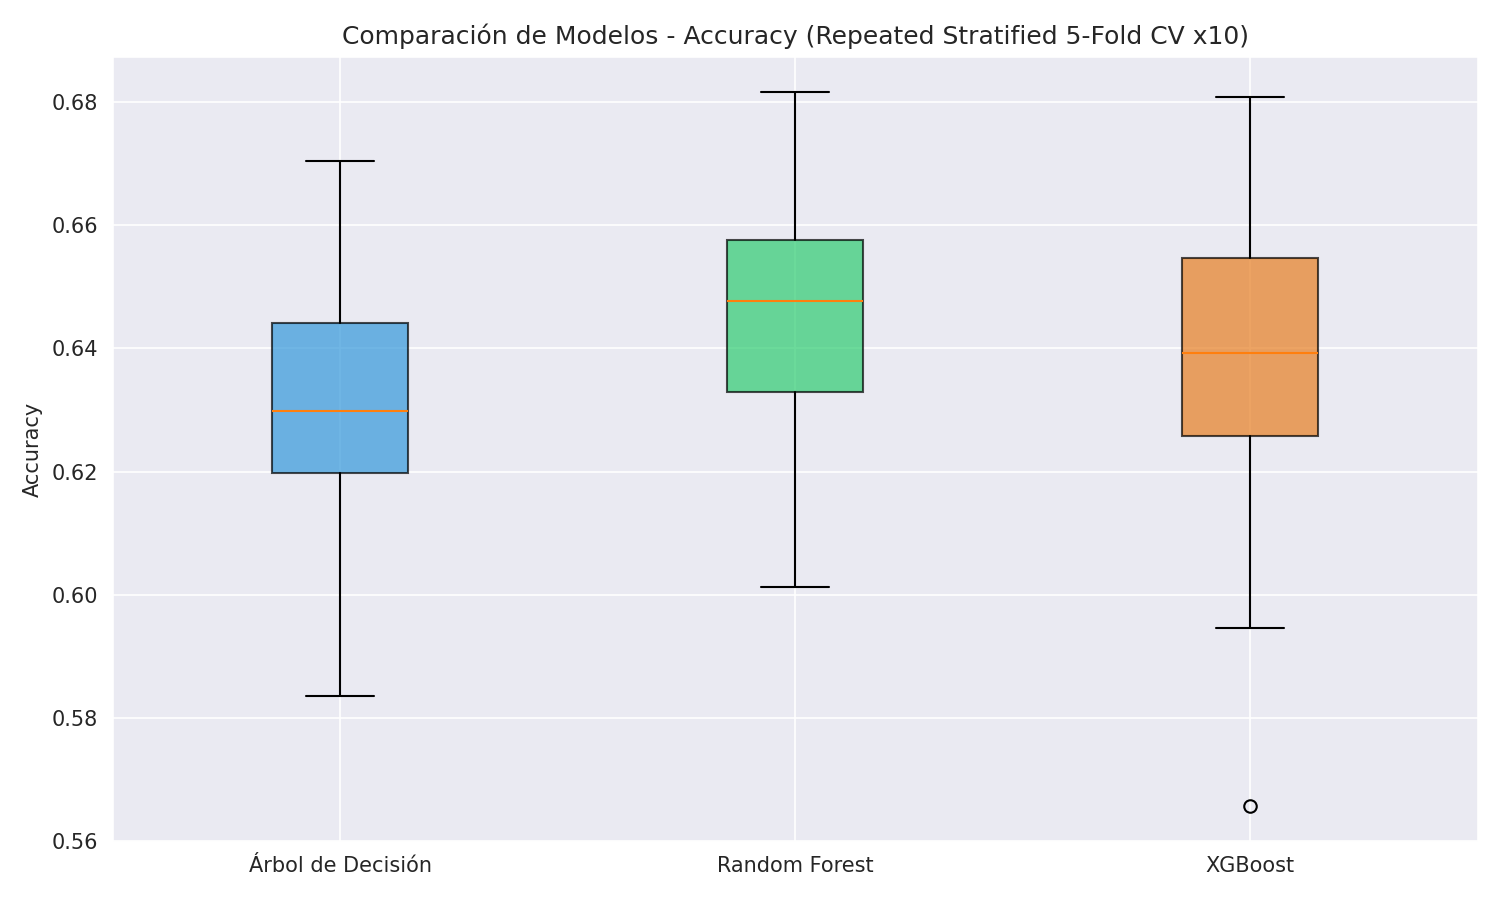
\includegraphics[width=0.75\textwidth]{figuras/fig13_comparacion_boxplots.png}
    \caption{Boxplots comparativos de Accuracy con validación cruzada repetida. Random Forest muestra la mediana más alta y menor dispersión.}
    \label{fig:comp_boxplots}
\end{figure}

\subsection{Curvas ROC}

\begin{figure}[H]
    \centering
    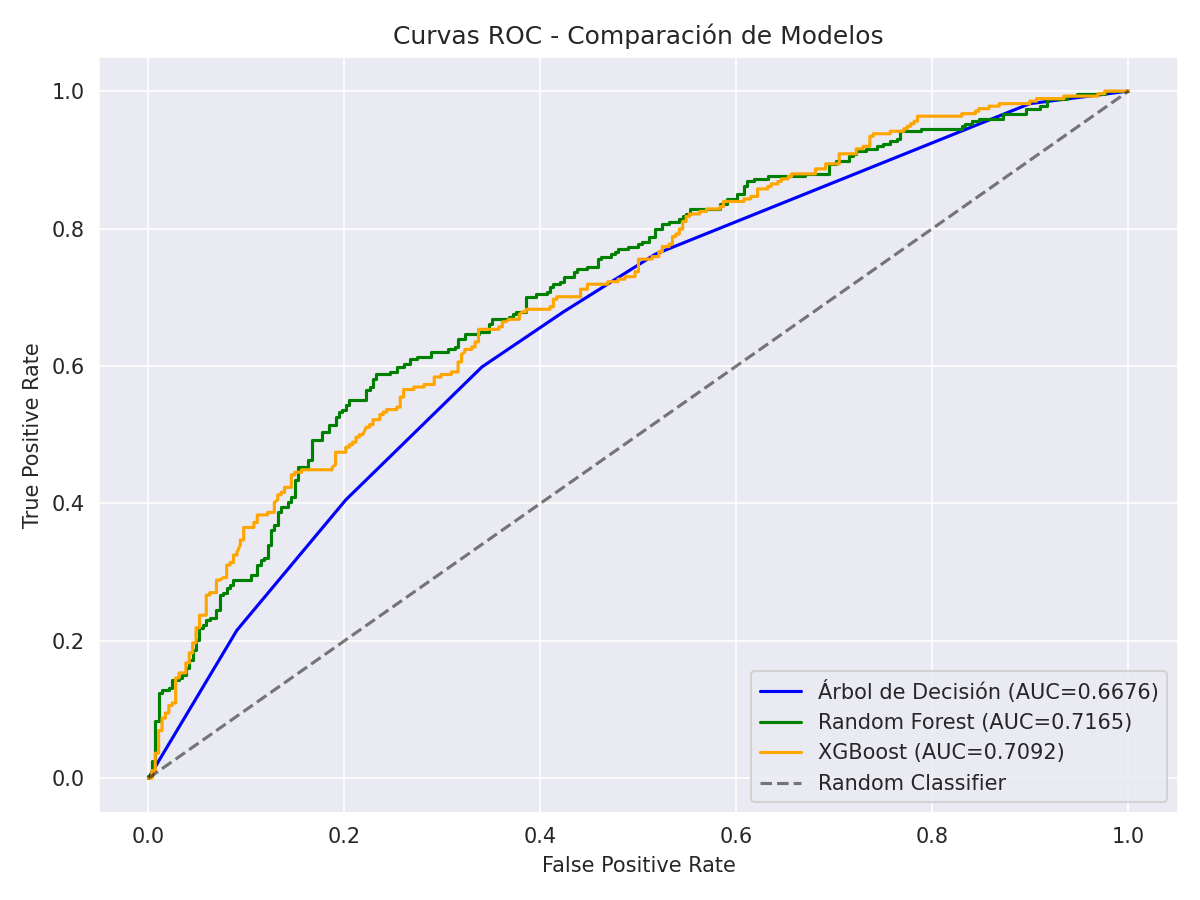
\includegraphics[width=0.65\textwidth]{figuras/fig14_comparacion_roc.png}
    \caption{Curvas ROC comparativas. Random Forest y XGBoost muestran un AUC superior al Árbol de Decisión.}
    \label{fig:comp_roc}
\end{figure}

\subsection{Matrices de confusión}

\begin{figure}[H]
    \centering
    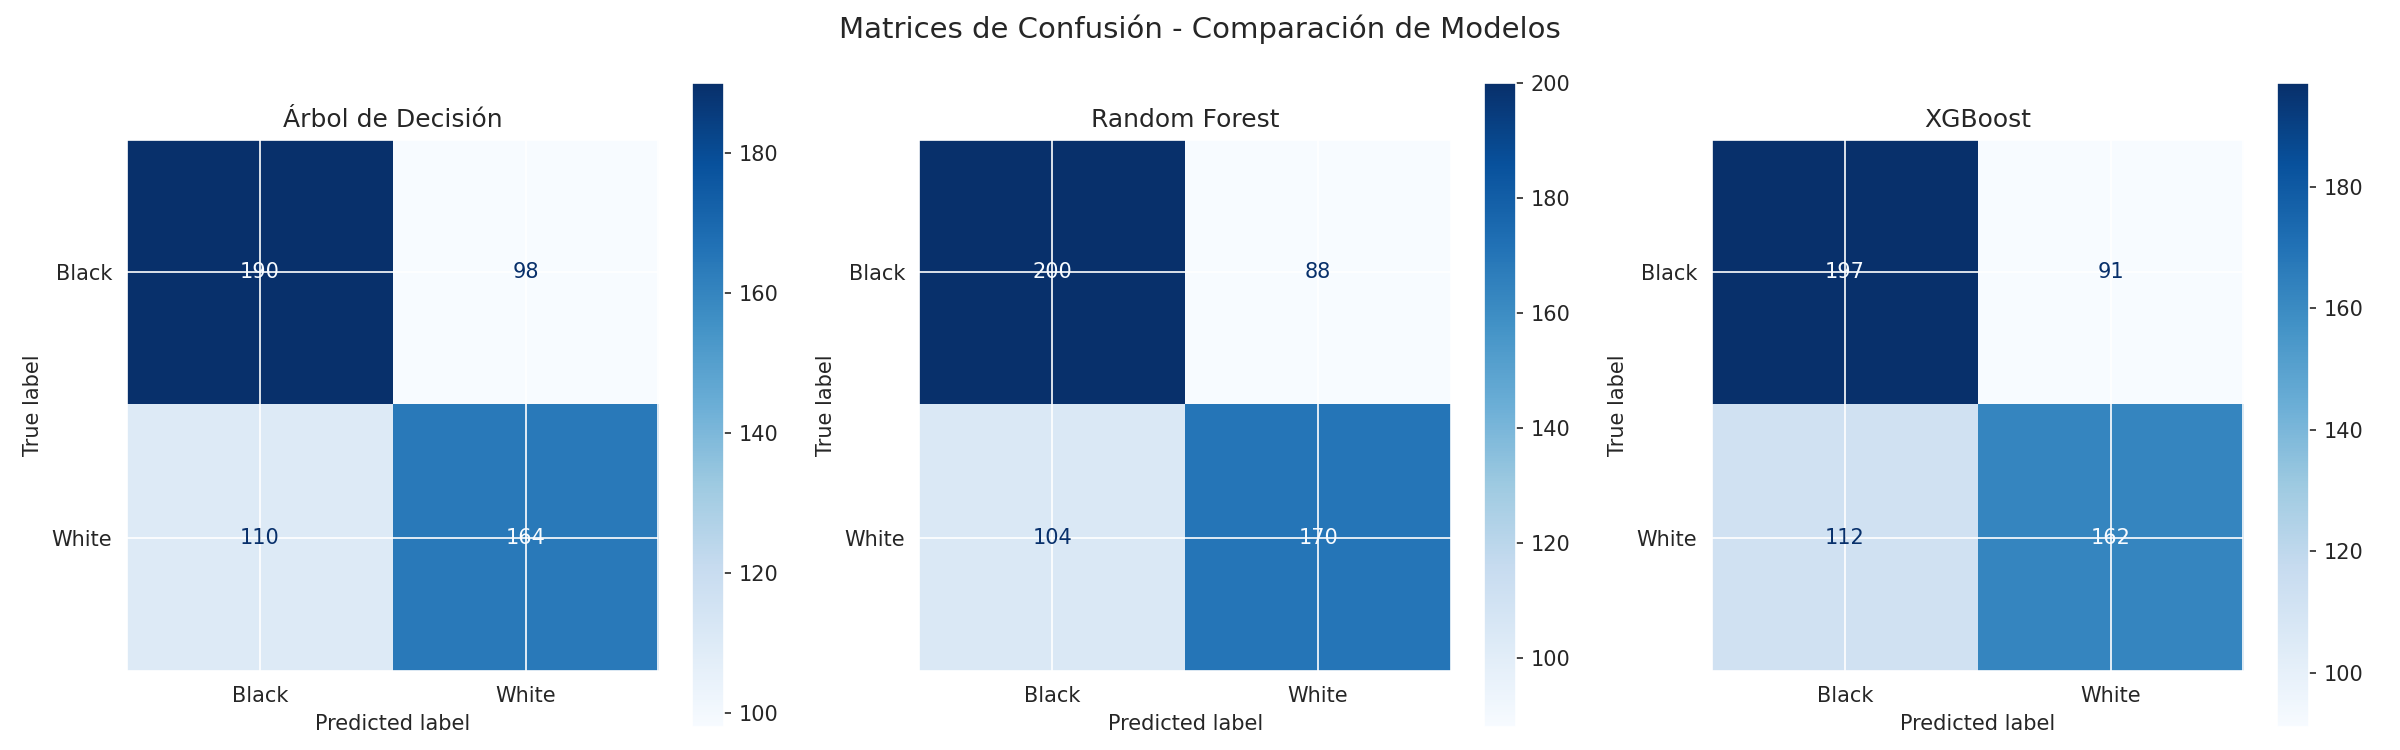
\includegraphics[width=\textwidth]{figuras/fig15_comparacion_confusion_matrices.png}
    \caption{Matrices de confusión comparativas en el conjunto de test.}
    \label{fig:comp_cm}
\end{figure}

\subsection{Importancia de variables comparativa}

\begin{figure}[H]
    \centering
    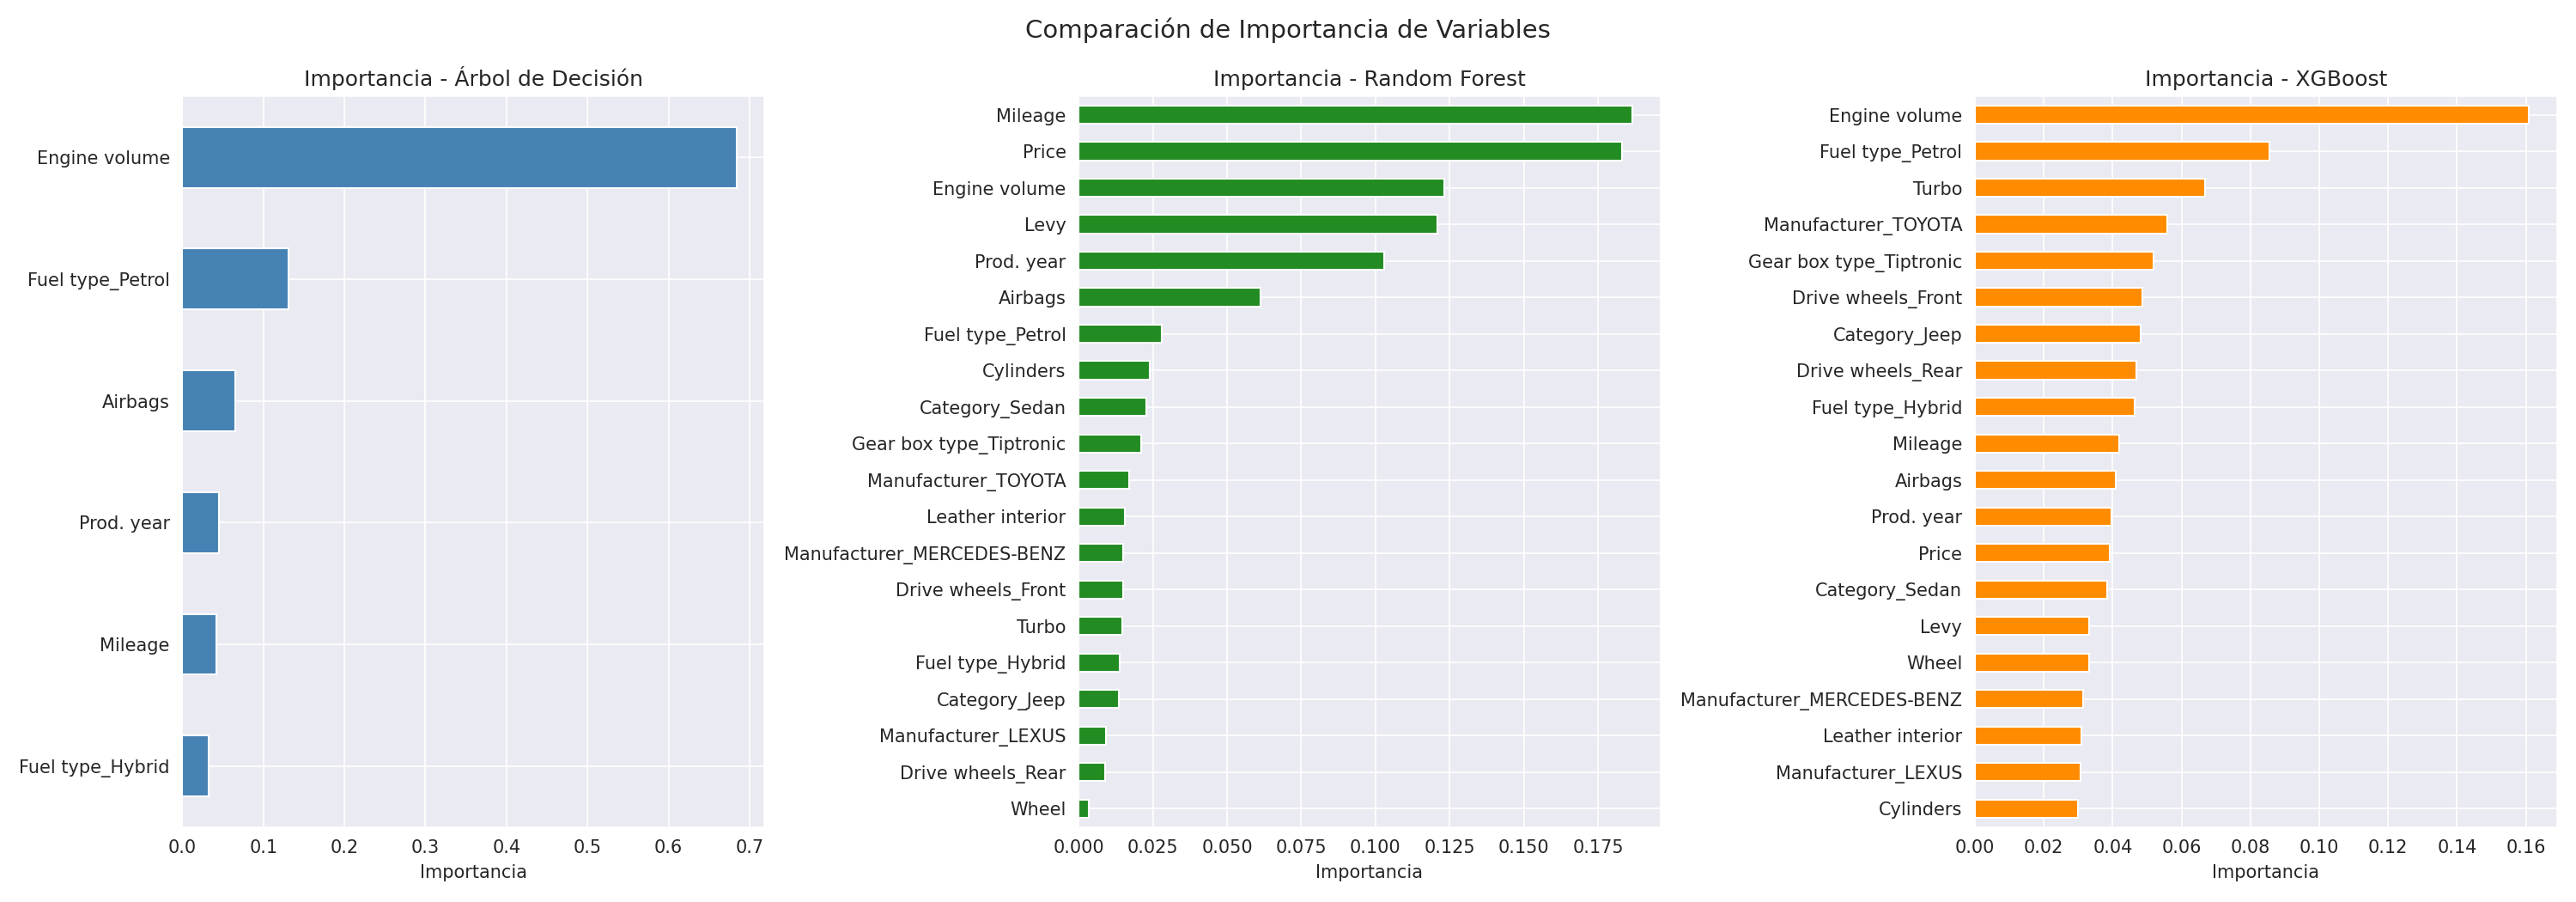
\includegraphics[width=\textwidth]{figuras/fig17_comparacion_feature_importance.png}
    \caption{Comparación de la importancia de variables entre los tres modelos.}
    \label{fig:comp_importance}
\end{figure}

El Árbol de Decisión concentra casi toda la importancia en \texttt{Engine volume} (68.4\%), mientras que Random Forest y XGBoost distribuyen la importancia de forma más equitativa entre las variables, destacando \texttt{Engine volume}, \texttt{Price}, \texttt{Mileage}, \texttt{Prod.\ year} y \texttt{Levy}.

\subsection{Conclusiones y selección del modelo final}

\begin{enumerate}
    \item \textbf{Random Forest} es el modelo con mejor rendimiento generalizado (\textbf{Accuracy test: 65.8\%, AUC: 0.717}), a pesar de mostrar cierto sobreajuste.
    \item \textbf{XGBoost} obtiene resultados intermedios (Accuracy test: 63.9\%, AUC: 0.709), con un sobreajuste algo menor gracias a la regularización.
    \item El \textbf{Árbol de Decisión} tiene la menor capacidad predictiva pero es el más interpretable y estable, sin sobreajuste apreciable.
    \item La tarea de predicción es inherentemente difícil: el color de un coche tiene una relación débil con sus características mecánicas, lo que explica las accuracies moderadas (63-66\%).
    \item \textbf{Modelo seleccionado: Random Forest}, por presentar el mejor balance entre capacidad predictiva (Accuracy, AUC) y robustez (menor desviación estándar en CV repetida).
\end{enumerate}

Si la interpretabilidad fuera prioritaria, el Árbol de Decisión sería preferible. No obstante, al priorizar la capacidad predictiva tal como solicita el enunciado, \textbf{Random Forest es la mejor elección}.

\end{document}
